\chapter{General Framework}
\label{chap:framework}

\section*{Introduction}
\addcontentsline{toc}{section}{Introduction}

This chapter sets the frame of the project: the host company and team, the context of the work, the existing solutions, the problems the project addresses, the solution we propose, its objectives, and the development process we followed, the Unified Process.

\section{Host organization}

\subsection{Presentation}

This graduation project was carried out within a work and study program (alternance) at \textbf{Capgemini Engineering} (Figure~\ref{fig:capgemini-logo}), the engineering and research and development branch of the Capgemini group. The group, headquartered in France, provides consulting, digital transformation and engineering services to many industries. The automotive sector is one of them, where Capgemini works both on software systems and on embedded engineering.

\begin{figure}[H]
\centering

\includegraphics[width=0.45\textwidth]{cover_capgemini_engineering.pdf}
\caption{Logo of Capgemini Engineering.}
\label{fig:capgemini-logo}
\end{figure}

\subsection{Department and work context}

The program takes place in the Automotive division of Capgemini Tunisia, within the Battery Management Systems (BMS) team, which develops and validates the embedded software of battery management functions for electric and hybrid vehicles. Since September 2024, it has combined a full time position in this team, five days a week from 9 am to 6 pm, as a quality assurance (QA) tester of battery management software for BMW Group, with classes at ESPRIT on Saturdays. A large part of this work consists in checking the messages that the \glspl{ecu} exchange on the \gls{can} bus: whether a cell voltage, a temperature or a state of charge is sent at the expected rate and with a plausible value.

CANvisionNative is not one of the team's deliverables: it was built alongside this position, from February 2026. The idea came from the difficulties met in this daily validation work. Working inside a team that knows \gls{ecu} communication and automotive embedded software helped keep the project close to real needs.

\section{Project context}

An electric vehicle relies on its \gls{can} bus to let its \glspl{ecu} exchange data, and the Battery Management System is one of the busiest of them: it sends cell voltages, temperatures, currents and the state of charge many times per second. Validating a BMS therefore means reading a large amount of \gls{can} traffic and deciding, frame after frame, whether it behaves as expected.

The \gls{can} protocol was designed for reliability on a closed network. It gives no sender identity and no authentication, and the security literature has shown that it can be abused through message injection, flooding or replay~\cite{koscher2010experimental,lokman2019intrusion}. A validation toolchain that does not watch the bus cannot notice a malicious frame any more than a faulty one.

In this context, an engineer needs to work on recorded logs as well as on a live bus, to replay a session after a change, to see quickly which frames depart from the usual behaviour of the vehicle, and to understand why.

\section{Study of existing solutions}
\label{sec:existing}

The existing solutions fall into three categories. Figure~\ref{fig:existing-logos} shows the commercial and open source tools and the diagnostic standards discussed below.

\begin{figure}[H]
\centering
\begin{tabular}{ccccc}
\techlogo[0.62cm]{vector.pdf}{CANoe, CANalyzer} & \techlogo{savvycan.png}{SavvyCAN} & \techlogo{linux.pdf}{candump (can-utils)} & \techlogo[1cm]{sae.pdf}{SAE J1979 (\acrshort{obd})} & \techlogo[1cm]{iso.pdf}{ISO 14229 (\acrshort{uds})} \\
\end{tabular}
\caption[Existing tools and diagnostic standards.]{Existing tools and diagnostic standards: Vector CANoe and CANalyzer, SavvyCAN, candump from the Linux can-utils, and the SAE J1979 and ISO 14229 standards used by diagnostic scanners.}
\label{fig:existing-logos}
\end{figure}

\subsection{CAN analysers}

Commercial tools such as Vector CANoe~\cite{vector_canoe} and CANalyzer are the professional standard for observing \gls{can} traffic: they capture raw frames, decode them with a \gls{dbc} file and replay a recorded log. They show what is on the bus, but not whether a frame is normal for this vehicle, unless custom scripts are written on top of the product.

\subsection{Intrusion detection research}

Research on \gls{can} intrusion detection~\cite{lokman2019intrusion} follows three families. \textbf{Signature based detection} compares the traffic with known attack patterns and cannot recognise a new one. \textbf{Specification based detection} writes the expected behaviour by hand for every vehicle. \textbf{Anomaly based detection} learns normal traffic, for example from the timing of the messages~\cite{song2016intrusion,cho2016fingerprinting} or from its entropy~\cite{muter2011entropy}, and flags what deviates from it. These detectors usually rely on one signal, aim at attacks rather than at explaining the bus, and are evaluated on public benchmarks~\cite{seo2018gids,verma2020road}.

\subsection{Viewers and diagnostic scanners}

Open source utilities such as candump~\cite{canutils} and SavvyCAN~\cite{savvycan} display raw frames, with little control over replay and no notion of what is abnormal. Diagnostic scanners based on \gls{obd}, defined in SAE~J1979~\cite{sae_j1979}, or on \gls{uds}, defined in ISO~14229~\cite{iso14229}, ask specific \glspl{ecu} for known parameters, so they only see what they ask for.

\subsection{Synthesis}

Table~\ref{tab:existing-comparison} summarises these categories.

\begin{table}[H]
\centering
\small
\caption{Existing solutions and their limits for BMS validation work.}
\label{tab:existing-comparison}
\begin{tabularx}{\textwidth}{|P{2.9cm}|P{2.9cm}|Y|Y|}
\hline
\textbf{Solution or category} & \textbf{Main purpose} & \textbf{Strengths} & \textbf{Limitations relevant to this project} \\
\hline
\gls{can} analysers (Vector CANoe, CANalyzer) & Observe, decode and replay \gls{can} traffic & Professional standard; capture, \gls{dbc} decoding and replay through a rich, configurable interface & No judgement on whether a frame is normal for the vehicle without custom scripts \\
\hline
Intrusion detection research & Detect attacks on the \gls{can} bus & Signature based: precise on known attacks; specification based: needs no attack data; anomaly based: learns normal traffic, widely applicable & Usually one signal or one set of rules; aims at attacks rather than at explaining the bus; a model trained on one vehicle rarely transfers; no explanation of an alert \\
\hline
Open source viewers (candump, SavvyCAN) & Display and log raw frames & Lightweight and open source & Little control over replay; no notion of what is abnormal \\
\hline
Diagnostic scanners (\gls{obd}, \gls{uds}) & Request known parameters, such as fault codes, from specific \glspl{ecu} & Standard request and response protocols & Only see what they ask for; do not monitor the bus as a whole \\
\hline
\end{tabularx}
\end{table}

Three limits come back. A detector built on a single signal misses a problem that does not disturb that signal. A model trained on one vehicle rarely transfers to another, because message layouts, sending rates and value ranges differ, and choosing the right model is often treated as a detail. And no tool turns an anomaly score into an explanation an engineer can act on within one workflow.

\section{Problem statement}

Four problems of day to day BMS validation work motivated the project:

\begin{enumerate}
    \item \textbf{No live view of the traffic:} Reading raw frames says what happened, not whether it should have happened. By the time something odd is noticed in a spreadsheet or a log viewer, the context that would explain it is often lost.
    \item \textbf{Weak replay:} Replaying a session is central to validation, but the usual tools either replay frames without judging them or accept only a few log formats, so engineers convert files by hand or change tools in the middle of an investigation.
    \item \textbf{Scattered tools:} No single tool available to the team combines decoding, replay, live capture and anomaly detection. An engineer combines a \gls{can} analyser, a diagnostic scanner, and a spreadsheet for comparisons across sessions.
    \item \textbf{Alerts without explanation:} When a tool flags something, it is usually a bare number that does not say which pattern caused it or what to check next.
\end{enumerate}

The lack of security of the \gls{can} protocol (ISO~11898~\cite{iso11898}) makes these problems worse. Security is therefore a real but secondary motivation: the first goal is one clear and explainable view of the bus. The question this project answers is therefore: how can we give a BMS engineer one view of the \gls{can} traffic, adapted to each vehicle, that explains its own alerts, and show that it works on real recordings?

\section{Proposed solution}
\label{sec:proposed-solution}

We propose \textbf{CANvisionNative}, a diagnostic and validation platform for the \gls{can} traffic of Battery Management Systems. Diagnostics is its main purpose; live monitoring, log replay and anomaly detection are the means to serve it. It is made of four parts:

\begin{itemize}
    \item A Windows desktop client (\gls{wpf}, \gls{mvvm}) where the analyst imports a log, replays it and reviews the results.
    \item A Python backend (FastAPI) that reads recordings in several formats, decodes the frames when a \gls{dbc} file exists, scores each frame and explains the flagged ones in plain language.
    \item Machine learning models trained separately for each vehicle.
    \item Three traffic sources: recorded logs, a live simulator, and live capture from a \gls{can} adapter.
\end{itemize}

CANvisionNative does not compete with detection research; it gathers in one diagnostic workflow what the tools of \Sref{sec:existing} offer separately: replay of several log formats, monitoring, anomaly detection per vehicle, and explanations in plain language. The model used for a vehicle is chosen explicitly and its status is shown before use. The platform can be used after the fact, on a recorded log, or as a live monitor when an adapter is connected.

\section{Objectives}

\subsection{General objective}

The general objective is to design, build and validate a diagnostic platform for Battery Management Systems that gives an engineer a unified view of the \gls{can} traffic, adapts to the vehicle being analysed, and explains its own alerts.

\subsection{Specific objectives}

The specific objectives are:

\begin{enumerate}
    \item Build a detection pipeline that combines a machine learning model with timing, payload and persistence checks.
    \item Accept the common recording formats (\gls{csv}, \gls{mf4}, candump, Vector and PCAN logs), a live simulator and live capture through python-can.
    \item Train a separate model for each vehicle, and put into production only the models evaluated on a recording kept out of their training.
    \item Build a desktop client to import a log, replay it, review the anomalies and export a report.
    \item Add an explanation layer, separate from detection, using rules and a \gls{llm}.
    \item Validate the pipeline on real recordings with reproducible evidence, and correct every defect found.
\end{enumerate}

\section{Development methodology}
\label{sec:methodology}

\subsection{Comparison: Waterfall, Scrum and the Unified Process}

Before organising the work, we compared three processes usually considered for a project of this size: the Waterfall model~\cite{royce1970managing}, Scrum~\cite{schwaber2020scrum}, and the \gls{up}~\cite{jacobson1999unified}, with its variant \gls{ttup}~\cite{roques2007uml}, which separates a functional branch and a technical branch before joining them in the design.

We chose the \gls{up}. Two main uncertainties of the project could not be estimated at the start: how well a model trained for one vehicle would perform, and how many defects a careful validation would uncover. A Waterfall plan would have frozen the detection design and the validation scope before either was known. Scrum assumes a team with separate roles and regular ceremonies, which one developer cannot reproduce. The \gls{up} keeps what fits a project of one person: iterations that each deliver a working increment, use cases that drive the work, an architecture tested early, and a list of risks that decides the order of the work.

Table~\ref{tab:methodology-comparison} compares the three processes on the criteria that mattered for this project.

\begin{table}[H]
\centering
\small
\caption{Comparison of Waterfall, Scrum and the Unified Process.}
\label{tab:methodology-comparison}
\begin{tabularx}{\textwidth}{|P{2.7cm}|Y|Y|Y|}
\hline
\textbf{Criterion} & \textbf{Waterfall} & \textbf{Scrum} & \textbf{Unified Process (2TUP)} \\
\hline
Organisation & Sequential phases, each finished before the next & Short sprints with a prioritised backlog & Four phases, each made of iterations \\
\hline
Requirements & Frozen at the start & Change freely from sprint to sprint & Captured as use cases, refined at each iteration \\
\hline
Architecture & Designed once, early & Emerges from the increments & Central: an executable architecture is built and tested early \\
\hline
Risks & Found late, at integration or test & Handled implicitly, sprint by sprint & Listed at the start; the riskiest parts are done first \\
\hline
Documentation and models & Heavy, produced at each phase & Light & UML models as the main artefacts \\
\hline
Team needed & Any & A team with separate roles and regular ceremonies & Scales from one developer to a team \\
\hline
Fit for this project & Poor: the model quality and the number of defects were unknown & Partial: one developer cannot run the ceremonies & Good: iterative, driven by use cases and risks, centred on the architecture \\
\hline
\end{tabularx}
\end{table}

\subsection{Principles and phases of the Unified Process}

The \gls{up}~\cite{jacobson1999unified,kruchten2003rup} rests on four principles:

\begin{itemize}
    \item \textbf{Driven by the use cases:} The use cases capture what the users need, and every iteration implements and tests some of them.
    \item \textbf{Centred on the architecture:} An executable architecture is built early and the rest of the system grows on it.
    \item \textbf{Iterative and incremental:} The work is cut into iterations, each one delivering a tested increment.
    \item \textbf{Driven by the risks:} The main risks are listed at the start, and the iterations are ordered so that the riskiest parts are tackled first.
\end{itemize}

The life of a project is divided into four phases, each closed by a milestone. \textbf{Inception} defines the vision, the scope, the main use cases and the risks. \textbf{Elaboration} analyses the requirements and builds the architecture baseline. \textbf{Construction} builds the system in iterations. \textbf{Transition} delivers the system to its users: final tests, deployment and documentation. In every phase, the work spans the same disciplines, in varying proportions: requirements, analysis and design, implementation, test and deployment.

\subsection{The Unified Process applied to CANvisionNative}

Table~\ref{tab:up-phases} and Figure~\ref{fig:project-timeline} show how the project followed these phases. The roadmap of the project listed eight milestones, M1 to M8: the live foundation, the hardware layer, the training of the vehicle models, the explanation engine, the real time charts, session recording, integration, and the decoding pipeline. The live foundation, M1, built the executable architecture of the elaboration phase. The construction phase was made of four iterations: the first delivered milestones M3 to M8; the second validated this first pipeline on a real recording and corrected its defects; the third delivered milestone M2, the hardware layer; and the fourth rebuilt the models and evaluated them on recordings they had never seen.

\begin{table}[H]
\centering
\small
\caption{Phases of the Unified Process in the project.}
\label{tab:up-phases}
\begin{tabularx}{\textwidth}{|P{2.6cm}|P{2.1cm}|Y|P{2.2cm}|}
\hline
\textbf{Phase} & \textbf{Period (2026)} & \textbf{Content and deliverables} & \textbf{Presented in} \\
\hline
Inception & February & Problem, existing tools, vision, use cases, initial risks and plan & Chapters~\ref{chap:framework} and~\ref{chap:inception} \\
\hline
Elaboration & February to March & Analysis and design models; executable architecture: client and backend, one runtime engine for replay, simulation and live capture (M1) & Chapter~\ref{chap:elaboration} \\
\hline
Construction, iteration 1 & March to June & First detection pipeline and client: M3 to M8 & \Sref{sec:it1} \\
\hline
Construction, iteration 2 & June to July & Validation and correction of six defects on a Kia EV6 recording & \Sref{sec:it2} \\
\hline
Construction, iteration 3 & August to September & Hardware layer and bench rig (M2) & \Sref{sec:it3} \\
\hline
Construction, iteration 4 & September & Model rebuild and evaluation on recordings kept out of training & \Sref{sec:it4} \\
\hline
Transition & September to October & Final release, tests, deployment guide and report & Chapter~\ref{chap:transition} \\
\hline
\end{tabularx}
\end{table}

\begin{figure}[H]
\centering
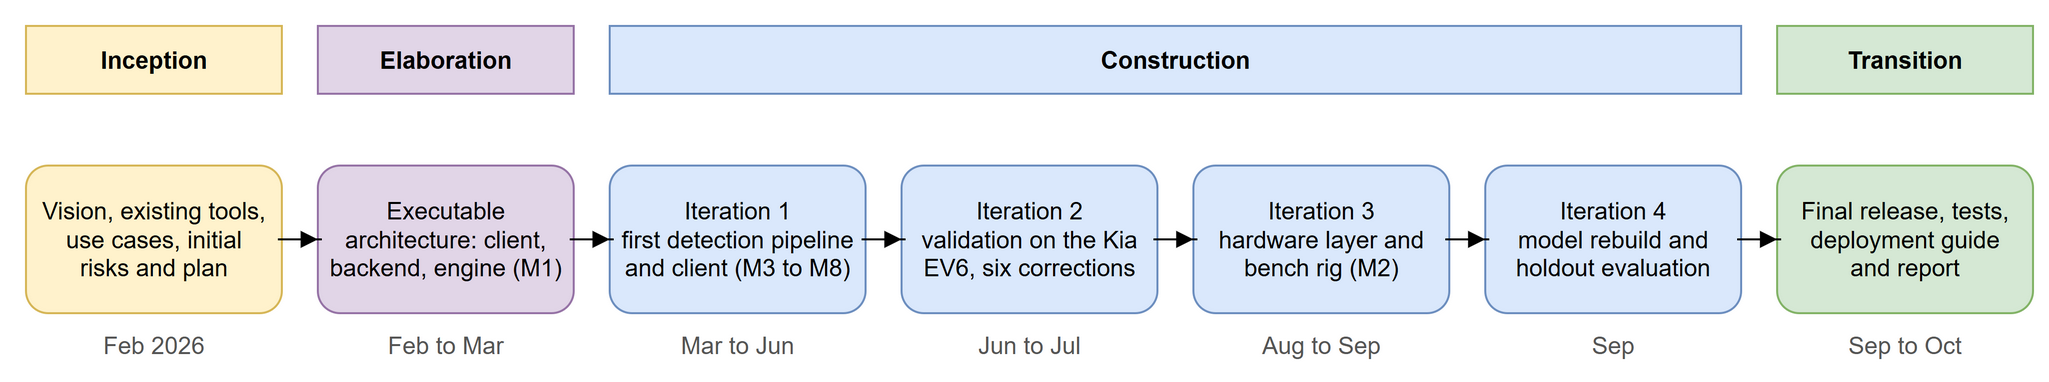
\includegraphics[width=\textwidth]{project_timeline.png}
\caption{Phases and iterations of the Unified Process in the project.}
\label{fig:project-timeline}
\end{figure}

Two rules applied to every iteration. A claim about the system was accepted only once shown on real data, and a defect was considered fixed only once the same test, run again, gave the expected result. As the only developer, we did not reproduce the roles of a team; each iteration ended with a review of its increment against its use cases before the next one started.

\subsection{Modelling language and tools}

The models of this report follow the \gls{uml}~\cite{omg2017uml}. The following diagrams are used:

\begin{itemize}
    \item \textbf{Use case diagram:} It shows the actors of the system and the services the system offers them.
    \item \textbf{Activity diagram:} It shows the flow of actions of a use case, with its decisions, divided between the actors and the system.
    \item \textbf{Class diagram:} It shows the classes of the software, with their attributes, their operations and the relations between them. The domain model, a class diagram of the concepts of the problem without software details, and the data model, which describes the tables of the database, are drawn in the same notation.
    \item \textbf{Component diagram:} It shows the parts of the system and the interfaces through which they depend on each other.
    \item \textbf{Deployment diagram:} It shows the machines and the processes on which the components run, and how they communicate.
    \item \textbf{Sequence diagram:} It shows, for one scenario, the numbered messages exchanged over time between an actor and the boundary, control and entity objects of the system.
    \item \textbf{State diagram:} It shows the states an object goes through and the events that move it from one state to another.
\end{itemize}

The diagrams were drawn with draw.io from a script that keeps every diagram in a file that can be edited. The source code was versioned with Git and GitHub, and the report was typeset with \LaTeX.

\section*{Conclusion}
\addcontentsline{toc}{section}{Conclusion}

This chapter presented the host company, the context of the project, the existing solutions and their limits, the problem and the solution we propose, its objectives, and the Unified Process that organised the work. The next chapter presents the inception phase: the capture of the requirements.
